\begin{minipage}{0.75\linewidth}
\begin{figure}[h]
    \centering
    \begin{adjustbox}{max width=1.0\linewidth, keepaspectratio}
        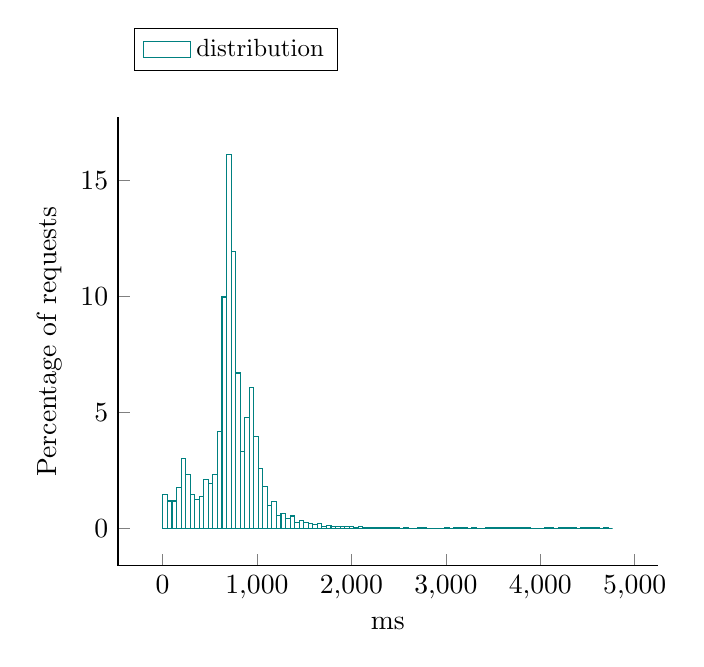
\begin{tikzpicture}
            \begin{axis}[ylabel = Percentage of requests, 
xlabel = ms, 
legend style = {nodes={scale=0.9, transform shape}, at={(0.03,1.2)}, anchor=north west, draw=black, fill=white, align=left, legend columns=3},
area style, mark size = 0pt,
 cycle list name = exotic,
  axis lines* = left]
		\addplot +[ybar interval] coordinates {
			 (5, 1.44686)
			 (53.09, 1.17623)
			 (101.18, 1.17623)
			 (149.27, 1.74872)
			 (197.36, 3.02904)
			 (245.45, 2.33163)
			 (293.54, 1.46768)
			 (341.63, 1.24909)
			 (389.72, 1.36359)
			 (437.81, 2.09222)
			 (485.9, 1.92568)
			 (533.99, 2.31082)
			 (582.08, 4.19486)
			 (630.17, 9.9823)
			 (678.26, 16.1237)
			 (726.35, 11.9496)
			 (774.44, 6.70345)
			 (822.53, 3.3309)
			 (870.62, 4.79858)
			 (918.71, 6.05808)
			 (966.8, 3.96586)
			 (1014.89, 2.58145)
			 (1062.98, 1.82159)
			 (1111.07, 0.988862)
			 (1159.16, 1.145)
			 (1207.25, 0.551681)
			 (1255.34, 0.634954)
			 (1303.43, 0.416363)
			 (1351.52, 0.530863)
			 (1399.61, 0.249818)
			 (1447.7, 0.322681)
			 (1495.79, 0.239409)
			 (1543.88, 0.197772)
			 (1591.97, 0.166545)
			 (1640.06, 0.218591)
			 (1688.15, 0.0832726)
			 (1736.24, 0.124909)
			 (1784.33, 0.0624545)
			 (1832.42, 0.0624545)
			 (1880.51, 0.0728635)
			 (1928.6, 0.0624545)
			 (1976.69, 0.0832726)
			 (2024.78, 0.0312272)
			 (2072.87, 0.0832726)
			 (2120.96, 0.0312272)
			 (2169.05, 0.0416363)
			 (2217.14, 0.0208182)
			 (2265.23, 0.0312272)
			 (2313.32, 0.0104091)
			 (2361.41, 0.0312272)
			 (2409.5, 0.0208182)
			 (2457.59, 0.0208182)
			 (2505.68, 0)
			 (2553.77, 0.0104091)
			 (2601.86, 0)
			 (2649.95, 0)
			 (2698.04, 0.0104091)
			 (2746.13, 0.0312272)
			 (2794.22, 0)
			 (2842.31, 0)
			 (2890.4, 0)
			 (2938.49, 0)
			 (2986.58, 0.0312272)
			 (3034.67, 0)
			 (3082.76, 0.0104091)
			 (3130.85, 0.0208182)
			 (3178.94, 0.0104091)
			 (3227.03, 0)
			 (3275.12, 0.0416363)
			 (3323.21, 0)
			 (3371.3, 0)
			 (3419.39, 0.0208182)
			 (3467.48, 0.0104091)
			 (3515.57, 0.0416363)
			 (3563.66, 0.0312272)
			 (3611.75, 0.0208182)
			 (3659.84, 0.0208182)
			 (3707.93, 0.0312272)
			 (3756.02, 0.0312272)
			 (3804.11, 0.0312272)
			 (3852.2, 0.0520454)
			 (3900.29, 0)
			 (3948.38, 0)
			 (3996.47, 0)
			 (4044.56, 0.0104091)
			 (4092.65, 0.0312272)
			 (4140.74, 0)
			 (4188.83, 0.0104091)
			 (4236.92, 0.0104091)
			 (4285.01, 0.0104091)
			 (4333.1, 0.0104091)
			 (4381.19, 0)
			 (4429.28, 0.0104091)
			 (4477.37, 0.0104091)
			 (4525.46, 0.0208182)
			 (4573.55, 0.0208182)
			 (4621.64, 0)
			 (4669.73, 0.0208182)
			 (4717.82, 0)
			 (4765.91, 0)
		};
\addlegendentry{distribution};
           \end{axis}
      \end{tikzpicture}
  \end{adjustbox}
  \caption{Response time distribution - req = ReadUser-3}
\end{figure}
\end{minipage}\hfill\begin{minipage}{0.18\linewidth}
\begin{table}[h]
\begin{tabular}{|cc|}
\hline
\textbf{} & \textbf{ms}\\ \hline
 \Xhline{0.005\arrayrulewidth}
min & 5\\
 \Xhline{0.005\arrayrulewidth}
max & 4814\\
 \Xhline{0.005\arrayrulewidth}
mean & 742\\
 \Xhline{0.005\arrayrulewidth}
std & 386\\
\hline
\hline
 \Xhline{0.005\arrayrulewidth}
25th & 625\\
 \Xhline{0.005\arrayrulewidth}
50th & 722\\
 \Xhline{0.005\arrayrulewidth}
75th & 888\\
 \Xhline{0.005\arrayrulewidth}
80th & 931\\
 \Xhline{0.005\arrayrulewidth}
85th & 971\\
 \Xhline{0.005\arrayrulewidth}
90th & 1040\\
 \Xhline{0.005\arrayrulewidth}
95th & 1210\\
 \Xhline{0.005\arrayrulewidth}
99th & 1997\\
\hline
\end{tabular}
\caption{Response time}
\end{table}
\end{minipage}\hfill